\section{Alignment of amino acid sequences}

Sometimes, during evolution, in a protein some amino acids may be replaced
by other amino acids, usually with similar properties. Some other times one or
more amino acids may be added or removed.

Therefore when aligning proteins (and also DNA) sequences we should consider
the possibility of amino acid substitution, but also insertions and deletions.
These alignment gaps are generally represented by a `` - ''.

How can we align sequences?
We require algorithms able to find the best alignment between two sequences,
allowing gaps and mismatches.
Problems:
\begin{itemize}
  \item We need an objective function to establish exactly what we want to
obtain
  \item We need an algorithm to find the best alignment, that is the alignment
that returns the highest score with the objective function. Alternatively, an
algorithm to find an alignment that approximate in the best possible way the
best alignment.
\end{itemize}

\subsection{Matches and mismatches have different weights}

We require algorithms able to find the best alignment between two sequences,
allowing gaps and mismatches.

Mismatches are not all the same. Some amino acids are very similar and can
replace each other with little consequences; other amino acids are very
different and should have different weight.

A logical consequence of the above is that also matches should have different
weight on the alignment.

\subsection{Objective function}

We need a computational evaluation of the alignment. First we need an objective
function to establish in mathematical terms what we want to obtain.
Then we need a suitable algorithm to find the alignment that maximizes the
value of the objective function.

The following \textbf{objective function} is generally used to align biological
sequences:

\begin{equation}
Score = \sum_{i=1}^{L} s(a_i,b_i) - \sum_{j=1}^{G} (\gamma + \delta(len(j)-1))
\end{equation}

Where:
\begin{itemize}
  \item \textbf{L} is the length of the alignment
  \item \textbf{G} is the length of the gap
  \item The \textbf{sum $s(a_i,b_i) (i=1..L) $} is calculated from the
\textbf{substitution matrix} $s$ that defines a score for every pair of aligned
amino acids.
  \item Then comes the \textbf{penalty for gaps}. Each penalty is calculated
 for each individual gap. \textbf{$\gamma$} is the fixed penalty for the
 opening of the gap and then there is a penalty proportional to to gap length
\textbf{$\delta$}.
\end{itemize}

\subsection{Substitution matrices}

A substitution matrix describes \textbf{the rate at which one character in a
sequence changes to other character states over time}.

Substitution matrices are usually seen in the context of amino acid or DNA
sequence alignments, where the similarity between sequences depends on their
divergence time and the substitution rates as represented in the matrix. \\

In a substitution matrix, the $(i,j)^{th}$ entry is equal to the probability of
the $i^{th}$ amino acid being transformed into the $j^{th}$ amino acid in a
certain amount of evolutionary time.

(Note that the identity matrix is also a substitution matrix) \\

The general idea (Margaret Dayhoff, 1978) was to start from the available
protein sequences (1500 sequences belonging to 71 families of closely related
proteins) and to calculate the probability in a small evolutionary step
(corresponding to 1\% of amino acid substitutions) that any amino acid would
change into another amino acid or remain the same.

Such matrix would be the PAM1 probability matrix, that is almost an identity
matrix with probability 0.99... for identities and 0.00... for substitutions.

The Smith–Waterman algorithm performs local sequence alignment; that is, for
determining similar regions between two strings of nucleic acid sequences or
protein sequences. Instead of looking at the entire sequence, the
Smith–Waterman algorithm compares segments of all possible lengths and
optimizes the similarity measure.

A PAM scoring matrix s is obtained from the PAM
probability matrix M and from the casual probability
matrix C, as indicated in the following equation:

\begin{equation}
s(a,b) = int(10*\frac{M(a,b)}{C(a,b)})
\end{equation}

\paragraph*{Blosum matrix}

The BLOSUM (BLOcks SUbstitution Matrix) matrix is a
substitution matrix used for sequence alignment of proteins.

BLOSUM matrices are used to score alignments between evolutionarily
divergent protein sequences. They are based on local alignments.

The BLOSUM matrices were produced from the BLOCK database, that contains
the sequence alignments of the most conserved regions of protein families.

These alignments are used to derive the BLOSUM matrices.

Only the sequences with a percentage of identity higher are used.

By using the block, counting the pairs of amino acids in each column of the
multiple alignment.

The procedure is similar to that used for PAM, but instead than reiterating
small evolutionary steps, with the Blosum matrix we consider actual blocks
with certain percentage of identity.

Therefore a Blosum100 does not make sense because it corresponds to an
identity matrix.

Very often people use Blosum60, obtained with blocks of 60\% identity.

The log ratio against the casual pairing is calculated in a way essentially
identical to that used for PAM.

\subsection{Smith-Waterman algorithm}

The algorithm requires:

\begin{itemize}
  \item two sequence $A = a_{1}a_{2}...a_{n}$ and $B = b_{1}b_{2}...b_{m}$ to
be aligned.
  \item $s(a,b)$, the similarity score
  \item $W_k$, the penalty of a gap that has length $k$
\end{itemize}

Then, it must be calculated a scoring matrix $H$ and initialize its first
row and first column.
The size of the scoring matrix is $(n + 1)*(m + 1)$ (Note the 0-based
indexing).

The first row and the first column must contain all zero.

The scoring matrix H must be filled with the rule shown in figure
\ref{fig:swalgorithm}

\begin{figure}[H]
  \centering
  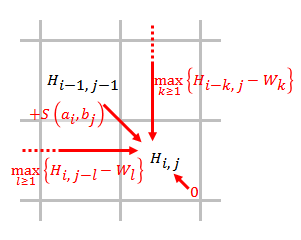
\includegraphics[scale=0.7]{SWalgorithm}
  \caption{Main rule of Smith-Waterman algorithm}
  \label{fig:swalgorithm}
\end{figure}

In other words, at every step it must be considered the highest value
of the column, of the row and then add the gap penalty. It must also
be considered the previous value on the diagonal and add the
similarity matrix corresponding value. These three values must be
compared and finally the highest value (or zero if there are only
negative value) must be chosen. \\

\textbf{Traceback}
Starting at the \textbf{highest score} in the scoring matrix H and ending at a
matrix cell that has a score of 0, traceback based on the source of
each score recursively generate the best local alignment.

\subsection{Application of few steps of the algorithm}

Take the alignment of DNA sequences \texttt{TGTTACGG} and
\texttt{GGTTGACTA} as an example.

Let the substitution matrices be the following:

\[ s(a_i,b_j) =
  \begin{cases}
    +3       & \quad \text{if } a_i = b_j\\
    -3	     & \quad \text{otherwise} \\
  \end{cases}
\]

And let the gap penalty be: \\

$W_k = k*W_1, W_1 = 2$ where k is the length of the gap. \\

Figure \ref{fig:steps} shows the scoring process of the first three elements.

\begin{figure}[H]
  \centering
  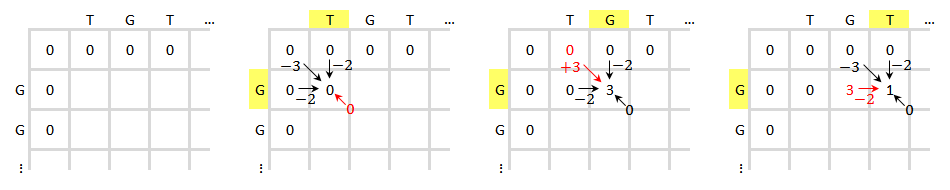
\includegraphics[scale=0.45]{Smith-Waterman-Example}
  \caption{few steps of Smith-Waterman algorithm}
  \label{fig:steps}
\end{figure}

\subsection{Properties of the Smith-Waterman algorithm}

\begin{itemize}
  \item It is based on dynamic programming
  \item It returns exactly the best alignment, given a suitable substitution
 matrix
  \item Its complexity is quadratic $\theta(n^2)$, more precisely
$\theta(n*m)$, where $n$ and $m$ are the lengths of the two sequences
  \item It can be used both on amino acid (proteins) and nucleic acid (DNA and
RNA) sequences
  \item In most cases we are not concerned in finding the best alignment
between 2 sequences, but in searching the most similar sequence in a database,
i.e. the sequence that can align with the highest score
  \item To search for similarities in a large database of sequences this
algorithm is too slow
\end{itemize}
